%% % para TCC edite arquivo /configs/preambuloTCC
% Versão Março de 2016
% Autor: Mauricio F. L Pereira
% e-mail: {mauricio, andreia.bonfante}@ic.ufmt.br
% 
%% MODELO DE MONOGRAFIA DO INSTITUTO DE COMPUTAÇÃO - UFMT


%% Abaixo são exemplos para cada tipo de trabalho 
%  Deixe apenas um dos \documentclass[]{} ativos, de acordo 
% com a fase (PTCC ou TCC ) e categoria (Graduação ou Especialização) 
% do seu trabalho de conclusão.
% Neste exemplo está ativado o exemplo de PTCC de Especialização em Banco de Dados
%% PTCC  (Especializacao, Banco de Dados)
%\documentclass[EspecializacaoPTCC,BD]{./configs/icufmt}

%% TCC  (Especializacao, Banco de Dados)
%\documentclass[EspecializacaoTCC,BD]{./configs/icufmt}

%% PTCC (Especializacao, Eng Web)
% \documentclass[EspecializacaoPTCC,EngWeb]{./configs/icufmt}

%% TCC (Especializacao, Eng Web)
%\documentclass[EspecializacaoTCC,EngWeb]{./configs/icufmt}

%% PTCC ( Graduacao Ciencia da Computação)
\documentclass[PTCC]{./configs/icufmt}

%% TCC ( Graduacao Ciencia da Computação)
%% \documentclass[TCC]{configs/icufmt}

\usepackage[brazil]{babel}

% para pacotes matemáticos
\usepackage{amsmath}
\usepackage{amsfonts}  
\usepackage{amssymb}  

%pacote para inclusão de códigos fonte
\usepackage{listings}

%pacote para lidar com tabelas com multiplas colunas
\usepackage{multirow}
	
% ---
% Pacotes adicionais, usados apenas para exemplos
% ---
\usepackage{lipsum}	% para geração de dummy text (pode ser comentado fora deste exemplo)
\usepackage{listings} % inclusão de códigos-fonte de diversas linguagens


%%%%%%%%%%%%%%%%%%%%%%%%%%%%%%%%%%%%%%%%%%%%%%%%%%%%%%%%%%%%%%%%%%%%%%%%%%%%%
%														    %
% INFORMAÇÕES SOBRE ORIENTADO E ORIENTADOR DO TRABALHO		%
%														    %
%%%%%%%%%%%%%%%%%%%%%%%%%%%%%%%%%%%%%%%%%%%%%%%%%%%%%%%%%%%%%%%%%%%%%%%%%%%%%

% Título do trabalho
\titulo{Título do Trabalho de Conclusão de Curso}

% Nome do autor do trabalho
\autor{Nome do autor}

% Exemplo de orientador de orientador e co-orientador (caso se aplique é 
% só descomentar a linha)
\orientador[Orientador:]{Prof. Dr. Fulano de Tal}

% Descomente se seu trabalho tem coorientador
% \coorientador[Coorientadora:]{Profa. Dra. Maria das Dores}

%%%%%%%%%%%%%%%%%%
%
%	MEMBROS DA BANCA DE AVALIAÇÃO DO TRABALHO
%
%%%%%%%%%%%%%%
% Avaliador externo 
\PrimeiroMembroBanca{\textbf{Prof. Dr. Mauricio Fernando Lima Pereira}}{Instituto de Computação - UFMT}
% Avaliador externo 
\SegundoMembroBanca{\textbf{Profa. Dra. Andreia Gentil Bonfante}}{Instituto de Computação - UFMT}
% Terceiro Avaliador (quando necessário)
%\TerceiroMembroBanca{\textbf{Prof. Dr. Josiel Maimone Figueiredo}}{Instituto de Computação - UFMT}

%% Data da defesa final do trabalho ( para preparação da folha de aprovação )
\DataDefesa{10}{de Dezembro}{2017}


% informações para organizar o pdf gerado no trabalho
% informações do PDF
\makeatletter
\hypersetup{
	%pagebackref=true,
	pdftitle={\@title}, 
	pdfauthor={\@author},
	pdfsubject={\imprimirpreambulo},
	pdfcreator={LaTeX com a classe IC-UFMT versao 2014},
	% % insira aqui suas palavras chaves relacionados ao seu trabalho
	pdfkeywords={abnt}{latex}{abntex}{abntex2}{trabalho acadêmico}, 
	colorlinks=false,       		% false: boxed links; true: colored links
	linkcolor=blue,          	% color of internal links
	citecolor=blue,        		% color of links to bibliography
	filecolor=magenta,      		% color of file links
	urlcolor=blue,
	bookmarksdepth=4
}
\makeatother

%compila o indice
\makeindex

%% iniciando o documento
\begin{document}
% Retira espaço extra obsoleto entre as frases.
% \frenchspacing 



% % % % % % %
%
%	ELEMENTOS PRÉ-TEXTUAIS
%
% % % % % % %

% descomente esse input caso esteja fazendo seu TCC
%% % % % % % %
%
%	ELEMENTOS PRÉ-TEXTUAIS
%
% % % % % % %

% folha de aprovação - ainda não utilizado neste modelo 
% deve ficar comentado
\begin{folhadeaprovacao}
	\begin{center}
	\cabecalhoCapa \\
    %\vspace*{\fill}
    \vspace{\stretch{2}}
	\textbf{CERTIFICADO DE APROVAÇÃO}
	\vspace{\stretch{2}} \\    
   \end{center}
	\begin{flushleft}   
	\hspace{1cm}\large\textbf{Título}: \imprimirtitulo
    \vspace{\stretch{2}} \\
   	\hspace{1cm}\large\textbf{Autor}: \imprimirautor
	\end{flushleft} 
    %\vspace*{\vfill}
% 	{\ABNTEXchapterfont\large\imprimirautor}		
% 		\vspace*{\fill}\vspace*{\fill}
% 		\begin{center}
% 			\ABNTEXchapterfont\bfseries\Large\imprimirtitulo
% 		\end{center}
% 		\vspace*{\fill}
		
% 		\hspace{.45\textwidth}
% 		\begin{minipage}{.5\textwidth}
% 			\imprimirpreambulo
% 		\end{minipage}%
% 		\vspace*{\fill}
	\begin{center}
    \vspace{\stretch{2}}
	\ImprimirDataDefesa
	\end{center}
    \begin{flushleft}
    \vspace{\stretch{1}}    
	\large Comissão examinadora: 
	\end{flushleft}
    \vspace{\stretch{2}}
	\assinatura{\textbf{\imprimirorientador} \\ Orientador}
    \vspace{\stretch{2}}
	\assinatura{\imprimirPrimeiroMembroBanca} 
    \vspace{\stretch{2}}
    \assinatura{\imprimirSegundoMembroBanca}
	%    \vspace{\stretch{2}}
	%	\assinatura{\imprimirTerceiroMembroBanca}


	
	\begin{center}
		\vspace*{0.5cm}
		{\large\imprimirlocal}
		\par
%		{\large\imprimirdata}
		\vspace*{1cm}
	\end{center}	
\end{folhadeaprovacao}

\pagenumbering{roman}
% dedicatória do trabalho
% ver arquivo dedicatoria.tex para ajustar o texto que irá aparecer aqui
% ----------------------------
% DEDICATÓRIA
% ----------------------------
\begin{dedicatoria}
	\vspace*{\fill}
	\flushright
	\begin{minipage}{0.54\textwidth}	
	\noindent
	% escreva entre os parêntesis o texto da sua dedicatória
	\textit{Este trabalho é dedicado a todos que um dia sonharam em se tornar cientistas.} 
	\end{minipage}
	\vspace*{\fill}
\end{dedicatoria}

% agradecimentos as pessoas que ajudaram no trabalho
% ver arquivo agradecimentos.tex para ajustar o texto que irá aparecer aqui
% ---
% Agradecimentos
% ---
\begin{agradecimentos}
	
	A todos que de alguma forma contribuíram para o desenvolvimento deste modelo de monografia.	
\end{agradecimentos}

% epigrafe do trabalho
% ver arquivo epigrafe.tex para ajustar o texto que irá aprecer aqui
% este é opcional
% ---
% Epígrafe
% ---
\begin{epigrafe}
	\vspace*{\fill}
	\begin{flushright}
		\textit{De tudo, ficaram três coisas:\\ \smallskip 
			A certeza de que estamos sempre começando...\\ \smallskip 
			A certeza de que precisamos continuar...\\\smallskip 
			A certeza de que seremos interrompidos antes de terminar...\\\medskip 
			Portanto devemos:\\\smallskip 
			Fazer da interrupção um caminho novo...\\\smallskip 
			Da queda um passo de dança...\\\smallskip 
			Do medo, uma escada...\\\smallskip 
			Do sonho, uma ponte...\\\smallskip 
			Da procura, um encontro...\\ }
		\textbf{Fernando Pessoa}
	\end{flushright}
\end{epigrafe}


% incluíndo o resumo do trabalho (em portugues)
% ver arquivo resumo.tex para ajustar o texto que irá aparecer aqui
% ---
% RESUMOS
% ---

% resumo em português
\setlength{\absparsep}{18pt} % ajusta o espaçamento dos parágrafos do resumo
\begin{resumo}
	O resumo deve ressaltar o objetivo, o método, os resultados e as conclusões do documento. A ordem e a extensão 	destes itens dependem do tipo de resumo (informativo ou indicativo) e do
	tratamento que cada item recebe no documento original. O resumo deve ser
	precedido da referência do documento, com exceção do resumo inserido no
	próprio documento. (\ldots) As palavras-chave devem figurar logo abaixo do
	resumo, antecedidas da expressão Palavras-chave:, separadas entre si por
	ponto e finalizadas também por ponto.
	
	\textbf{Palavras-chaves}: latex. abntex. editoração de texto.
\end{resumo}

% incluíndo o resumo do trabalho (em inglês)
% ver arquivo abstract.tex para ajustar o texto que irá aparecer aqui
% não necessário em trabalho de conclusão para curso de graduação
% resumo em inglês
\begin{resumo}[Abstract]
 \begin{otherlanguage*}{english}
   This is the english abstract.

   \vspace{\onelineskip}
 
   \noindent 
   \textbf{Keywords}: latex. abntex. text editoration.
 \end{otherlanguage*}
\end{resumo}

%
% e depois edite os arquivos :
%	- dedicatoria.tex
%	- agradecimentos.tex, 
%	- epigrafe.tex 
%	- resumo.tex 
%	- abstract.tex


% ---
% inserir o sumario
% ---
\pdfbookmark[0]{\contentsname}{toc}
\tableofcontents*
\cleardoublepage
% ---

% ---
% inserir lista de figuras
% ---
\pdfbookmark[0]{\listfigurename}{lof}
\listoffigures*
\cleardoublepage


% ---
% inserir lista de tabelas
% ---
\pdfbookmark[0]{\listtablename}{lot}
\listoftables*
\cleardoublepage



% ---
% inserir lista de abreviaturas e siglas
% organizar manualmente a ordem alfabetica
% ---
\begin{siglas}
	\item [ABNT] Associação Brasileira de Normas Técnicas
	\item [ARM] \textit{Advanced RISC Machine}
	\item [AT] Transformada de Anscombe
	\item [IC]Instituto de Computação
	\item [ULA] Unidade Lógica e Aritmética
	\item[UFMT]Universidade Federal de Mato Grosso
\end{siglas}
% ---


% ---
% inserir lista de símbolos
% ---
\begin{simbolos}
	\item[$ \Gamma $] Letra grega Gama
	\item[$ \Lambda $] Lambda
	\item[$ \zeta $] Letra grega minúscula zeta
	\item[$ \in $] Pertence
	\item [$\Delta t$] Variação de tempo	
	\item [$\omega_\alpha$]Variação do ângulo no sentido no passo $\alpha$	%
	\item [$P(\phi,t)$] Probabilidade de detecção de $\phi$ fótons em um tempo t de exposição
\end{simbolos}


% ----------------------------------------------------------
% ELEMENTOS TEXTUAIS (não remover ou alterar
% ----------------------------------------------------------
\textual
\setcounter{page}{1}
\pagenumbering{arabic}


%%%%%%%%%%%%%%%
%
%	Início dos capítulos 
%
%%%%%%%%%%%%%%%%%%%%%%%%%%

% iniciando a inclusão de capítulos
% pode-se organizar em arquivos .tex separados
% como apresenta o exemplo
\chapter{Introdução}
A Introdução anuncia o que se pretende dizer. Deve resumir o tema-problema a ser abordado, sua contextualização, o raciocínio a ser seguido na solução e os métodos a serem adotados, deixando claros o objetivo do trabalho, sua relevância, a justificativa da abordagem do seu tema, as propostas formuladas e a composição do trabalho. O leitor
deve ter uma ideia geral clara a respeito do que vai ler, após percorrer a introdução. 

É onde se faz a apresentação do problema, ressaltando os motivos mais importantes que levaram à abordagem do tema. O tema ou problema de pesquisa deve responder a o que vai ser investigado. A escolha do tema não é criação individual do aluno, mas é feita com base em obras que o abordem, trabalhadas por outros autores. A perspectiva adotada deve, contudo, ser diferente, a partir da consulta à documentação para a realização do projeto. O tema escolhido deve ser tratado como um problema a ser resolvido. O desenvolvimento do trabalho visa demonstrar uma posição única a respeito do tema problematizado. Trata-se de definir os aspectos de dificuldade e de se esclarecer os limites dentro dos quais a pesquisa e o raciocínio se desenvolverão.

Para decidir sobre o tema, algumas questões precisam ser respondidas, tais como:

\begin{itemize}
\item O tema é de interesse científico?
\item É um assunto a ser provado ou resolvido?
\item É um assunto que pode ser investigado?
\item Há a disponibilidade de material bibliográfico sobre o assunto?
\item Estou familiarizado com o tema?
\item A pesquisa é viável, em termos de tempo e recursos disponíveis?
\end{itemize}

O problema, por sua vez, é manifestação da vontade de investigar o tema, consistindo-se em uma questão não resolvida.

Exemplo: A adoção da técnica XYZ de avaliação pode corrigir os problemas com a evolução no aprendizado do aluno?

A Introdução deve conter:

1.1 Objetivo Geral

1.2 Objetivos Específicos

1.3 Justificativa

1.4 Metodologia

1.5 Cronograma Proposto

\section{Objetivo Geral}

O aluno expõe os objetivos que o trabalho visa atingir, relacionados com a contribuição
que pretende trazer. Os objetivos visam responder para que o trabalho será realizado.
Os objetivos devem ser formulados com verbos no infinitivo.

O \textbf{Objetivo Geral} expõe a razão maior do trabalho, ou o que se pretende com a realização do trabalho. A formulação do \textbf{objetivo gera}l usa verbos que admitem interpretações amplas, como \textbf{comprovar}, \textbf{desenvolver},
\textbf{entender}, \textbf{conhecer} e
\textbf{aperfeiçoar}.

Exemplo: O objetivo geral deste trabalho é estabelecer processos de apoio ao desenvolvimento das aplicações Web, adaptados à natureza dessas aplicações e tomando como base os aspectos observados na literatura sobre as características
dessas aplicações.

\section{Objetivos Específicos}
Os Objetivos Específicos relacionam os resultados que se pretende alcançar, na forma de etapas a serem cumpridas para a realização do objetivo geral. Os objetivos específicos são o ponto de partida para a investigação, ordenados
em uma sequência lógica de obtenção dos resultados desejados.
Os verbos para formular objetivos específicos devem admitir poucas interpretações, tais como \textbf{identificar}, \textbf{implementar}, \textbf{investigar}, \textbf{relacionar}, \textbf{escrever} e \textbf{aplicar}.

Exemplo:
\begin{itemize}
 \item Pesquisar sobre a evolução das arquiteturas de sistemas Web;
 \item Estudar as diferentes visões arquiteturais;
 \item Definir critérios para comparar as arquiteturas estudadas;
\end{itemize}

\section{Justificativa}

As justificativas devem ser baseadas na relevância social e científica da pesquisa proposta. Nesta etapa é respondido \textbf{porque} o trabalho será feito. A justificativa deve deixar claro para o leitor:

\begin{itemize}
 \item O estágio de desenvolvimento em que o tema se encontra e a sua evolução histórica;
\item O contexto em que o fenômeno ocorre;
\item A importância social e científica da realização da pesquisa sobre o tema.
\end{itemize}


\section{Metodologia}

Aqui se anuncia, para o projeto, o tipo de pesquisa que será desenvolvida, bem como os métodos e técnicas que serão adotados. Este item visa responder às questões sobre \textbf{como} o trabalho será feito,\textbf{ com o que},
\textbf{onde} e \textbf{com quem} será realizado.
Exemplo: O trabalho será desenvolvido a partir de pesquisa bibliográfica e de campo, através de método indutivo, utilizando levantamento de dados feito em entrevistas com professores e coordenadores acadêmicos, $\ldots$



\section{Cronograma}

A divisão da pesquisa em etapas de desenvolvimento, a partir dos objetivos específicos,requer que seja estabelecido um tempo para a execução cronológica dos trabalhos, dentro dos prazos estabelecidos para tal no calendário acadêmico. A elaboração do
cronograma responde à pergunta sobre \textbf{quando} cada fase do trabalho terá lugar. As etapas do cronograma devem cobrir todo o período de realização do trabalho de monografia, desde o refinamento do Projeto de Monografia até a apresentação do
trabalho monográfico à banca de avaliação. Cada etapa a ser cumprida deve ser exibida como uma linha na tabela que compõe o cronograma. As etapas são descritas após a exibição da tabela, tal qual mostra a tabela \ref{tab:Cronograma}.

\textbf{Exemplo}:

\begin{table}[h]
\caption{Cronograma Proposto}
\begin{tabular}{|c|c|c|c|c|c|c|c|c|c|c|c|c|c|c|c|c|}
\hline
& \multicolumn{16}{c|}{\textbf{Meses/Semanas}} \\
\hline
\multirow{2}{*}{\textbf{Etapas}} & \multicolumn{4}{c|}{\textbf{Mês 1}} & \multicolumn{4}{c|}{\textbf{Mês 2}} & \multicolumn{4}{c|}{\ldots} & \multicolumn{4}{c|}{\textbf{Mês N}}  \\
\cline{2-17}
        & 1 & 2 & 3 & 4 & 1 & 2 & 3 & 4 & 1 & 2 & 3 & 4 & 1 & 2 & 3 & 4 \\
\hline        
Etapa 1 & X & X & X & X &   &   &   &   &   &   &   &   &   &   &   &  \\
\hline 
Etapa 2 &   &   &   & X & X & X &   &   &   &   &   &   &   &   &   &  \\ 
\hline
Etapa 3 &   &   &   &   &   &   & X & X & X &   &   &   &   &   &   &  \\
\hline 
\ldots  &   &   &   &   &   &   &   &   &   & X & X & X & X & X & X &  \\ 
\hline
Etapa N &   &   &   &   &   &   &   &   &   &   &   &   &   &   &   & X \\
\hline 
\end{tabular}
\label{tab:Cronograma}
\end{table}
\begin{description}
\item [\textbf{Etapa 1}] - Exemplo: Pesquisa bibliográfica
Consiste da leitura de livros sobre o tema...
\item [\textbf{Etapa 2}] - Exemplo: Estudo de Caso
\ldots
\item[\textbf{Etapa N}] - Exemplo: Apresentação à banca avaliadora
\end{description}


\section{Estudo de Caso}
...

% 
\chapter{Fundamentação Teórica}
\thispagestyle{empty}
Aqui se forma um quadro teórico de princípios e conceitos, dentro do qual o Projeto de Monografia se baseia e se desenvolve. Este quadro teórico deve formar uma unidade lógica compatível com o tratamento do problema e com o raciocínio desenvolvido. Ele nem sempre precisa constar do trabalho final, com o mesmo grau de profundidade adotado para o Projeto de Monografia, uma vez que seja mantida a coerência entre o desenvolvimento realizado e o projeto.

É onde se desenvolve a ideia anunciada, através da discussão dos elementos teóricos e empíricos. A Fundamentação Teórica pode ser composta por subcapítulos, tópicos e sub-tópicos, identificados por títulos que forneçam a ideia exata do seu conteúdo. Nesta parte do trabalho as ideias são descritas, classificadas e definidas, as ideias conflitantes são comparadas, e a argumentação apropriada à natureza do trabalho é aplicada.

É importante observar que os conteúdos apresentados por outros autores devem ser referenciados no texto de acordo com as normas ABNT NBR 6023 e NBR 10520 

\chapter{Trabalho Desenvolvido}

Insira neste capítulo seu trabalho
No projeto, serão trabalhos iniciais, se vocês os tiver

\chapter{Resultados e discussões}

Insira neste capítulo os seus resultados e as discussões a respeito deles.
No projeto, serão resultados iniciais, se vocês os tiver

\chapter{Conclusões}

Insira aqui as conclusões do seu trabalho.

% ----------------------------------------------------------
% ELEMENTOS PÓS-TEXTUAIS
% ----------------------------------------------------------
\postextual

\bibliography{refs}


% ----------------------------------------------------------
% Apêndices
% ----------------------------------------------------------

% ---
% Inicia os apêndices
% ---
\begin{apendicesenv}
	
\chapter{Exemplo de apêndice}

Elemento opcional, que consiste em um texto ou 
documento elaborado pelo autor, a fim de complementar sua argumentação,  sem prejuízo da unidade nuclear do trabalho. 

Abaixo incluí algumas linhas aleatórias geradas pelo \LaTeX

\lipsum[2-9]


\chapter{Exemplo de códigos-fonte}

Neste capítulo é apresentado como inserir códigos-fontes no trabalho. Para isso é necessário a utilização do pacote listings, que foi adicionado no arquivo principal da monografia.

Exemplo de código java


\lstset{language=java}
\lstinputlisting{exemplo.java}


\pagebreak
Outro exemplo de como inserir código com caixa para caption

\lstset{
language = C, % Linguagem de programação
basicstyle = \footnotesize, % Tamanho da fonte do código
numbers = left, % Posição da numeração das linhas
numberstyle = \tiny\color{blue}, % Estilo da numeração de linhas
stepnumber = 1, % Numeração das linhas ocorre a cada quantas linhas?
numbersep = 10pt, % Distância entre a numeração das linhas e o código
backgroundcolor = \color{white}, % Cor de fundo
showspaces = false, % Exibe espaços com um sublinhado
showstringspaces = false, % Sublinha espaços em Strings
showtabs = false, % Exibe tabulação com um sublinhado
frame = single, % Envolve o código com uma moldura, pode ser single ou trBL
rulecolor = \color{black}, % Cor da moldura
tabsize = 2, % Configura tabulação em x espaços
captionpos = b, % Posição do título pode ser t (top) ou b (bottom)
breaklines = true, % Configura quebra de linha automática
breakatwhitespace= false, % Configura quebra de linha
title = \lstname, % Exibe o nome do arquivo incluido
%caption = \lstname, % Também é possível usar caption no lugar de title
keywordstyle = \color{blue}, % Estilo das palavras chaves
commentstyle = \color{green}, % Estilo dos Comentários
stringstyle = \color{red}, % Estilo de Strings
escapeinside = {\%*}{*)}, % Permite adicionar comandos LaTeX dentro do seu código
morekeywords     ={*,...} % Se quiser adicionar mais palavras-chave
}
\begin{lstlisting}{Exemplo de Caption de Código}
#include <stdio.h>

int main()
{
// declaracao de variavel
int c;
printf("Entre com o valor: ");
scanf("%i", &c);
printf("Res: %i", i*i);
}
\end{lstlisting}

\end{apendicesenv}

% ----------------------------------------------------------
% Anexo
% ----------------------------------------------------------

% ---
% Inicia os anexos
% ---
\begin{anexosenv}

% ---
%%% exemplo de uso de siglas e tabela de simbolos (podem ser incluídas em qualquer local do texto ou qualquer capítulo 
%%% simbolos utilizados neste capítulo


\chapter{Comandos Latex Básicos }
\thispagestyle{empty}
\section{Criando seções e capítulos}

Para criar capítulos deve-se utilizar o comando 
\begin{verbatim}
\chapter{ titulo do capitulo}                                               
\end{verbatim} 
e  para criar seções utiliza-se o comando 
\begin{verbatim}
\section{nome da secao} 
\end{verbatim}
 
\subsection{Criando uma subseção}

Subseções são criadas utilizando-se o comando
\begin{verbatim}
\subsection{nome da subsecao} 
\end{verbatim}

\section{Conceito de ambiente \LaTeX }

O conceito de ambiente em \LaTeX é semelhante ao de qualquer linguagem de
programação. Existe um comando que abre um escopo e outro que fecha

Assim sempre que se define \verb|begin{comando}| e \verb|end{comando}| se cria
um ambiente.

Os ambientes mais utilizados são

\begin{itemize}
\item center
\item figure
\item table
\item tabular
\item enumerate 
\end{itemize}
%
dentre outros. Nas seções seguintes veremos cada um desses ambientes.




%\section{Incluindo uma figura}

O comando que permite incluir uma figura é \verb|\includegraphics{nomeDoArquivo}|

Assim é possível incluir uma figura como um elemento do texto.

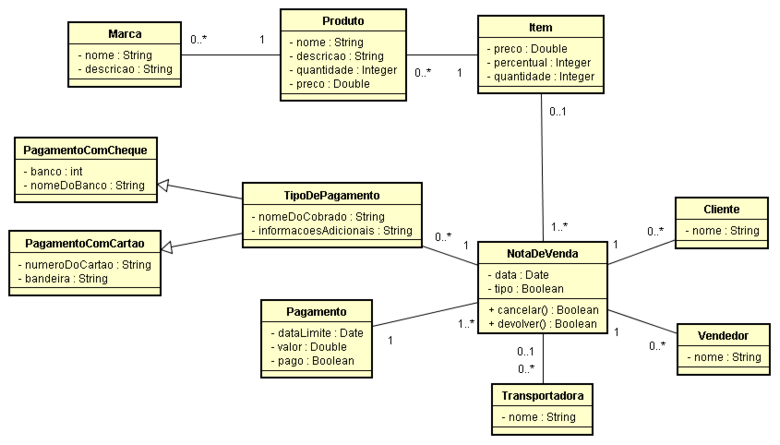
\includegraphics[width=0.9\textwidth]{modelo1}

Inserindo dentro do ambiente \textbf{figure} é possivel adicionar uma legenda e
uma referencia cruzada para se poder citar a figura dentro do texto
utilizando-se o comando \verb|\ref{rotulo}|. Repare que
está figura aparece na lista de figuras.

\begin{figure}[!hb]
\centering
\includegraphics[scale=0.4]{interface1} 
\caption{Exemplo de caption - legenda para uma figura}
\label{fig:interface}
\end{figure}

O código \LaTeX que permite incluir esta fígura é

\begin{verbatim}
\begin{figure}[!hb]
\centering
\includegraphics[scale=0.4]{figuras/interface1} 
\caption{Exemplo de caption - legenda para uma figura}
\label{fig:interface}
\end{figure} 
\end{verbatim}
                             

A Figura \ref{fig:interface} foi colocada dentro do ambiente  como um objeto do
texto. Da forma como ela está sendo referenciada, terá sua numeração feita de
forma automática

\section{Incluindo uma tabela}

A inserção de tabelas é feita utilizando-se o comando \verb|tabular|

Tal qual a figura, pode-se criar tabela dentro do ambiente \verb|table| ou fora.
Dentro do ambiente \verb|table|, a tabela poderá ter um caption e um rótulo.

\begin{tabular}{|l|c|r|p{4cm}|}
\hline
Id & Configuração & Valor & Benefícios \\
\hline
1 & Config 1 & 30.000,00 & Suporte gratis por 1 ano \\
\hline	
2 & Config 2 & 55.000,00 & Suporte gratis por 3 ano \\
\hline
\end{tabular}

A mesma tabela quando colocada em um ambiente \verb|table| aparece como Tabela
\ref{tab:TabEquipamentos}.

\begin{table}[h]
\centering
\caption{Tabela de aquisição de equipamentos de informática}
\begin{tabular}{|l|c|r|p{4cm}|}
\hline
Id & Configuração & Valor & Benefícios \\
\hline
1 & Config 1 & 30.000,00 & Suporte grátis por 1 ano \\
\hline	
2 & Config 2 & 55.000,00 & Suporte grátis por 3 ano \\
\hline
\end{tabular} 
\label{tab:TabEquipamentos}
\end{table}

O código \LaTeX que gera a Tabela \ref{tab:TabEquipamentos} é 

\begin{verbatim}
\begin{table}[h]
\centering
\caption{Tabela de aquisição de equipamentos de informática}
\begin{tabular}{|l|c|r|p{4cm}|}
\hline
Id & Configuração & Valor & Benefícios \\
\hline
1 & Config 1 & 30.000,00 & Suporte grátis por 1 ano \\
\hline	
2 & Config 2 & 55.000,00 & Suporte grátis por 3 ano \\
\hline
\end{tabular} 
\label{tab:TabEquipamentos}
\end{table}
\end{verbatim}


Exemplo do uso de multicoluna e multilinha

\begin{table}[!h]
\caption{Tabela fictícia com uso de comandos multicolumn e  multirow}
\begin{center}
\begin{tabular}{|l|c|c|c|c|}
\hline
 \multirow{2}{*}{Ano} & \multicolumn{2}{|c|}{Ciência da Computação}&
\multicolumn{2}{|c|}{Sistemas de Informação} \\ 
\cline{2-5}
& Homens & Mulheres & Homens & Mulheres \\
\hline
2009 & 36 & 4 & 37 & 3 \\
\hline
2010 & 39 & 1 & 37 & 3 \\
\hline
\end{tabular}
\end{center}
\label{tab:Ficcao1}
\end{table}

\begin{verbatim}
\begin{table}[!h]
\caption{Tabela fictícia com uso de comandos multicolumn e  multirow}
\begin{center}
\begin{tabular}{|l|c|c|c|c|}
\hline
\multirow{2}{*}{Ano} & \multicolumn{2}{|c|}
{Ciência da Computação}& \multicolumn{2}{|c|}{Sistemas de Informação} \\ 
\cline{2-5}
& Homens & Mulheres & Homens & Mulheres \\
\hline
2009 & 36 & 4 & 37 & 3 \\
\hline
2010 & 39 & 1 & 37 & 3 \\
\hline
\end{tabular}
\end{center}
\label{tab:Ficcao1}
\end{table}
\end{verbatim}

\section{Listas}

É possível criar diferentes tipos de listas em um texto. A seguir são mostrados
três tipos.

\subsection{Listas enumeradas}

As listas enumeradas são geradas utilizando o comando enumerate como mostrado a
seguir, onde a numeração é colocada de forma automatica

\begin{verbatim}
\begin{enumerate}
\item Primeiro item 
\item Outro item 
\item Novo Item
\end{enumerate} 
\end{verbatim}


Este código gera a lista enumerada 

\begin{enumerate}
\item Primeiro item 
\item Outro item 
\item Novo Item
\end{enumerate}

\subsection{Listas de itens}

As listas de itens servem para separar difentes itens sem numeração. Assim a
mesma lista acima pode ser colocada como 

\begin{itemize}
\item Primeiro item 
\item Outro item 
\item Novo Item
\end{itemize}


O código \LaTeX que gera esta lista é 

\begin{verbatim}
\begin{itemize}
\item Primeiro item 
\item Outro item 
\item Novo Item
\end{itemize} 
\end{verbatim}




\subsection{Listas personalizadas}

Também se pode criar marcadores personalizados na lista tal como é mostrado a
seguir

\begin{itemize}
\item [a)]Primeiro item 
\item [b)]Outro item 
\item [c)]Novo Item
\end{itemize}


O código \LaTeX que gera esta lista é 

\begin{verbatim}
\begin{itemize}
\item [a)]Primeiro item 
\item [b)]Outro item 
\item [c)]Novo Item
\end{itemize}
\end{verbatim}

\section{Inserindo fórmulas}

É possível introduzir formulas matemáticas de diferentes formas. Dentro do
texto, por exemplo pode-se colocar $\alpha = cos(\theta) + \log(x)$ com o comando

\verb|$\alpha = cos(\theta)+ \log(x)$|

Para que a fórmula aparece com destaque no texto, mas sem numeração deve-se
colocar a formula utilizando \verb|$$\alpha = cos(\theta)+ \log(x)$$|. Para a fórmula
acima aparecer em destaque  $$\alpha = cos(\theta) + \log(x)$$

Equações numeradas podem ser criadas utilizado-se o ambiente equation. Veja os
exemplo a seguir com o comando \LaTeX que gerou a equação mostrado em seguida.


\begin{equation}
  K_{m} = \sum_{i=1}^{m} i^2
  \label{eq:FormulaX}
\end{equation}
%
\begin{verbatim}
\begin{equation}
  K_{m} = \sum_{i=1}^{m} i^2
  \label{eq:FormulaX}
\end{equation}
\end{verbatim}


Várias equações como no exemplo da equação \ref{eq:FormulaY}
\begin{eqnarray}
x & = & 2\pi + b \nonumber\\
	&	= & 2\pi + 30  	
\label{eq:FormulaY}
\end{eqnarray}

Matrizes 

$$det(X) = \left|\begin{array}{ccc} 
1 & 2 & 3 \\
4 & 5 & 6 \\
7 & 8 & 9 \\
\end{array} \right| 
$$

\begin{verbatim}
$$det(X) = \left|\begin{array}{ccc} 
1 & 2 & 3 \\
4 & 5 & 6 \\
7 & 8 & 9 \\
\end{array} \right| 
$$
\end{verbatim}






\section{Incluindo referências}

Para incluir citações a outros trabalhos deve-se incluir o arquivo que contém as referências bibliográficas. Em geral este arquivo é incluído no arquivo de projeto como um último capítulo tal qual mostrado a seguir:

\begin{verbatim}
\begin{document}
\maketitle
\tableofcontents
\listoffigures
\listoftables
\listadesimbolos
\listadesiglas
\include{Agradecimentos}
%%% -------- incluindo capitulos que estão em arquivos separados
\include{Introducao}
\include{ExemploLatex}
%%%% -------- incluindo o arquivo de referências bibliografica (referencias.bib)
\bibliography{referencias}
\end{document}
\end{verbatim}

\section{Citações de trabalhos}

Os comandos \verb|\cite{chaveReferencia}| para citação \verb|\citeonline{chaveReferencia}|

Na linhas a seguir vamos apresentar exemplos de citações com diferentes números de autores, para melhor visualização.

Citação de trabalho com \textbf{um} autor: Um bom trabalho começo para aprender \LaTeX  é utilizar \cite{Knuth1984}.

Citação  de trabalho com \textbf{dois} autores: Um bom livro de processamento de imagens \cite{Gonzales2000}.

Citação  de trabalho com \textbf{três} autores ou mais: Trabalho com 3 autores \cite{Pereira2001}. Trabalho de tomografia no campo (4 autores) \cite{macedo2002wood}

Nas próximas linhas vamos discutir como citar trabalhos de outras formas

Citação on line. No trabalho desenvolvido por \citeonline{Knuth1984} pode-se encontrar alguma documentação importante a respeito do ambiente Latex. 

Um exemplo do uso de apud \apud{Unser1997}{macedo2002wood}


\section{Criando listas de índices}

A criação de listas em \LaTeX é muito simples 

Para criar um sumário pode-se utilizar o comando \verb|\tableofcontents|.

Para criar uma lista de figuras deve-se utilizar o comando \verb|\listoffigures|.

Para criar uma lista de tabelas deve-se utilizar o comando \verb|\listoftables|.

Para criar um resumo pode-se utilizar o comando 
\begin{verbatim}
\begin{abstract}
Texto do resumo
\end{abstract}
\end{verbatim}

\section{Personalizando a monografia}

\subsection{Ajustando titulo, orientador e autor}

Comando para ajustar o título: 

\noindent
\verb|\title{Teste de escrita de monografia para apresentação na Especialização}|

Comando para ajustar o nome do orientador

\verb|\orientador{Prof. Dr. Fulano de Tal}|

Comando para ajustar o autor

\verb|\author{Nome do autor}|




% ---
%\lipsum[30]


\end{anexosenv}


\end{document}

